\documentclass[12pt,a4paper,oneside]{book}
\usepackage[utf8]{inputenc}
\usepackage[english]{babel}
\usepackage[T1]{fontenc}
\usepackage[hidelinks]{hyperref}
\usepackage{amsmath}
\usepackage{amsfonts}
\usepackage{amssymb}
\usepackage{algorithm}
\usepackage[noend]{algpseudocode}
\usepackage{listings}
\usepackage{pdfpages}
\usepackage{indentfirst}
\usepackage{titlesec}
\usepackage{tocloft}
\usepackage{setspace}
\usepackage{siunitx}
\usepackage{graphicx}
\usepackage{tabularx}
\usepackage{array}
\usepackage{multirow}
\usepackage{threeparttable}
\usepackage{fixltx2e}
\graphicspath{ {./figures/} }
%\usepackage{natbib}
\usepackage[left=3.5cm,right=2cm,top=2.5cm,bottom=2.5cm]{geometry}
\setstretch{1.5} %riadkovanie 1.5
\titleformat{\chapter}{\normalfont\huge\bfseries}{\thechapter}{20pt}{\normalfont\huge\bfseries}
\setcounter{tocdepth}{3}
\setcounter{secnumdepth}{3}
\newtheorem{definition}{Definition}

\newcommand\mytitle{Software for isometric gene tree reconciliation}
\newcommand\mythesistype{Master's thesis}
\newcommand\myauthor{Bc. Dominika Mihálová}
\newcommand\myadvisor{doc. Mgr. Bronislava Brejová, PhD.}
\newcommand\myplacedate{Bratislava, 2021}
\newcommand\myuniversity{COMENIUS UNIVERSITY IN BRATISLAVA}
\newcommand\myfaculty{FACULTY OF MATHEMATICS, PHYSICS AND INFORMATICS}
\newcommand{\sub}[1]{$_{\text{#1}}$}
\newcommand{\reference}[1]{č.~\ref{#1}}
\newcommand{\imageHeight}{150px}
\renewcommand{\cftchapleader}{\cftdotfill{\cftdotsep}}

\begin{document}
\sloppy
%obal
\frontmatter
\thispagestyle{empty}
\noindent
\begin{minipage}{\textwidth}
	\begin{center}
		\textbf{\myuniversity \\
		\myfaculty}
	\end{center}
\end{minipage}

\vfill
\begin{center}
	\begin{minipage}{0.8\textwidth}
		\centering{\textbf{\Large\MakeUppercase{\mytitle}}} \\
		\centering{\mythesistype}
	\end{minipage}
\end{center}
\vfill
2020 \hfill
\myauthor
\eject 

%titulná strana
\thispagestyle{empty}
\noindent
\begin{minipage}{\textwidth}
	\begin{center}
		\textbf{\myuniversity \\
		\myfaculty}
	\end{center}
\end{minipage}
\vfill

\begin{center}
	\begin{minipage}{0.8\textwidth}
		\centering{\textbf{\Large\MakeUppercase{\mytitle}}} \\
		\centering{\mythesistype}
	\end{minipage}
\end{center}
\vfill
\begin{tabular}{l l}
	Study programme: & Applied Computer Science\\
	Field of study: & Computer Science\\
	Department: & Department of Computer Science\\
	Supervisor: & \myadvisor
\end{tabular}
\vfill
\noindent
\myplacedate \hfill
\myauthor
\eject 

%zadanie - pojde obrazok
%\chapter*{Thesis assignment}
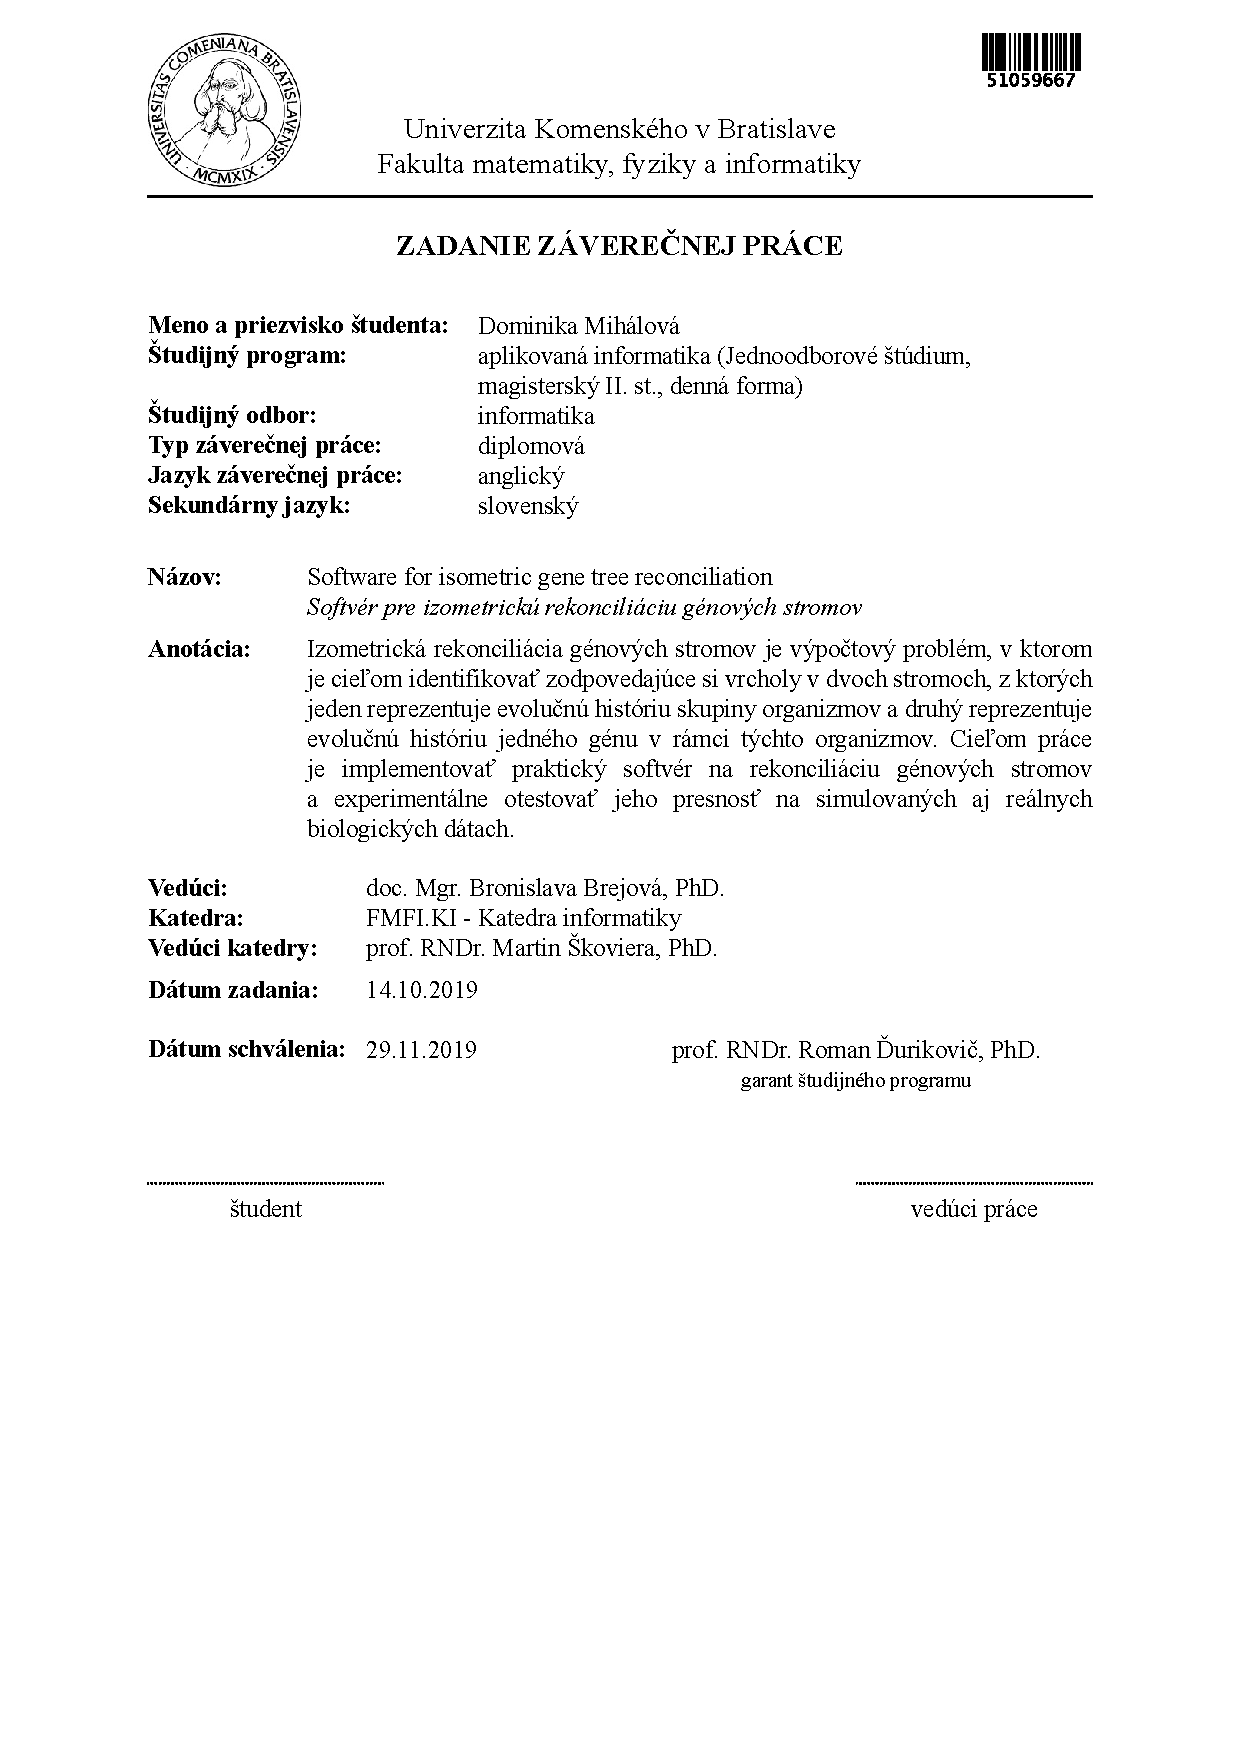
\includepdf{zadanie-zp.pdf}
\vfill\eject 

%sk abstrakt
\chapter*{Abstrakt}

Cieľom diplomovej práce bolo implementovať softvér pre izometrickú rekonciliáciu génových stromov a experimentálne otestovať jeho presnosť na simulovaných aj reálnych biologických dátach. Práca je rozdelená do piatich kapitol.

Prvá kapitola je venovaná základnej terminológií z oblasti bioinformatiky a prehľadu rôznych prístupov k riešeniu problému rekonciliácie s názornými riešeniami tejto problematiky v podobe softvérov.

Ďalšia časť uvádza algoritmy a implementovaný softvér. Opisujú sa vytvorené algoritmy, špecifikujú sa vlastnosti implementovaného softvéru, spôsob spracovania vstupov a následné výstupy.

Štvrtá kapitola prezentuje testovaciu sadu a opisuje vykonané experimenty na implementovanom softvéri pre izometrickú rekonciliáciu.

Záverečná kapitola sa zaoberá interpretáciou výsledkov testovania implementovaného softvéru. 
\\\\
\textbf{Kľúčové slová:} izometrická rekonciliácia génového stromu, nepresné dĺžky hrán, fylogenetický strom
\vfill\eject 

%en abstrakt
\chapter*{Abstract}

The main goal of the diploma thesis was to implement software for isometric gene tree reconciliation and to experimentally evaluate its accuracy on simulated and real biological data. The thesis is divided into five chapters.

The first chapter presents the basic terminology in the field of bioinformatics and an overview of different approaches to solving the problem of reconciliation with concrete solutions to this problem in the form of software.

The next section presents algorithms and implemented software. The created algorithms are described, the properties of the implemented software, the method of input processing and subsequent outputs are specified.

The fourth chapter presents a test set and describes the experiments performed on the implemented software for isometric reconciliation.

The final chapter deals with the interpretation of the results of testing the implemented software.
\\\\
\textbf{Keywords:} isometric gene tree  reconciliation, inexact branch lengths, phylogenetic tree
\vfill\eject  

%zoznam obrazkov
\listoffigures
\newpage

%obsah
\tableofcontents
\newpage

\mainmatter

%úvod
\chapter*{Introduction}
\addcontentsline{toc}{chapter}{Introduction}
\vfill\eject

\input chapter_1_overview.tex
\input chapter_2_algorithms.tex
\input chapter_3_implementation.tex
\input chapter_4_experiments.tex
\input chapter_5_results.tex

\backmatter

%záver
\chapter*{Conclusion}
\addcontentsline{toc}{chapter}{Conclusion}
\vfill\eject 

%príloha
\chapter*{Appendix}
\addcontentsline{toc}{chapter}{Appendix}
\vfill\eject 



\nocite{*}
\bibliographystyle{plain}
\bibliography{bibliography}

\end{document}